[Теорема о пределе композиции]\label{tpk}
Пусть $\lim\limits_{x\to a}f(x)\hm=b$, $\lim\limits_{y\to b}g(y)\hm=c$; $a$, $b$, $c$, вообще говоря,
 принадлежат расширенной числовой прямой: $a,b,c\in\ol{\R}$.

$\a$пустое место$\s$ "--- потом, когда мы придём к~дурным выводам, оно перестанет быть пустым.

Тогда куда же будет стремиться: $\lim\limits_{x\to a}g\big(f(x)\big)\hm=c$ "--- получалось, надо сказать, враньё. Почему:

Например: $g(y)\hm=\begin{cases}
    1,&y\neq0;\\
    0,&y\hm=0.
\end{cases}$ Пусть $f(x)\equiv 0$ "--- вообще тривиальная функция (рис. \ref{rkomp}).

$f(x)\xrightarrow[x\to 0]{}0$ тождественный ноль везде стремится к~нулю,     $g(y)\xrightarrow[y\to 0]{}1$, а~вот $g\big(f(x)\big)\equiv 0\xrightarrow[x\to 0]{}0$. Ну с~чем связаны все проблемы? на~внешнюю функцию никак не влияет значение $x\hm=a$.

\begin{figure}[htbp]\centering
    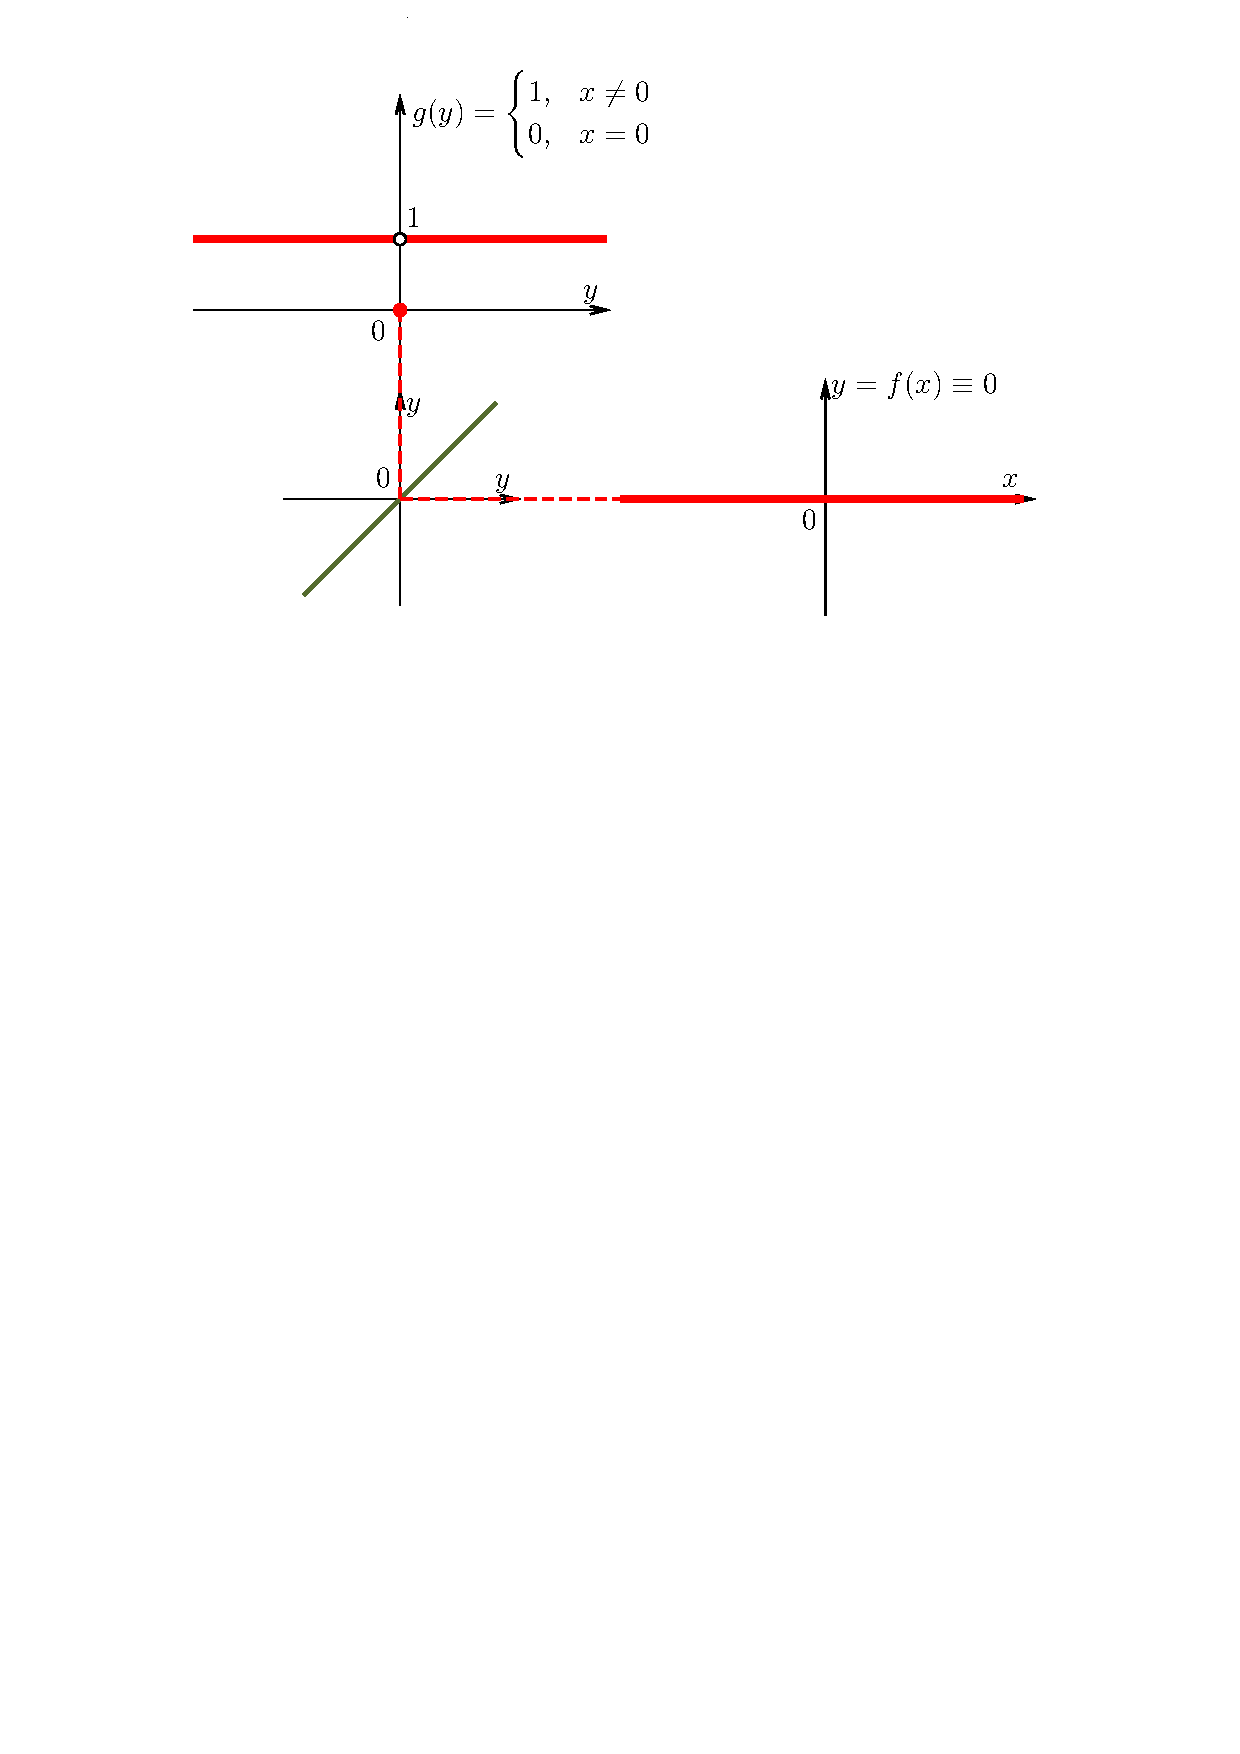
\includegraphics[height=6cm]{img/final/galat/vvedf/graf.pdf}\\ \caption{Разрывная композиция} \label{rkomp}
\end{figure}

Самое время в~$\a$пустое место$\s$ поставить: пусть выполняется хотя бы одно из~следующих утверждений:

\begin{enumerate}\renewcommand{\theenumi}{\asbuk{enumi}}\renewcommand{\labelenumi}{\theenumi)}
    \item\label{a} $g(b)$ определена и равна $c$;
    \item\label{b} $f(x)$ не принимается значения $b$ в~некоторой проколотой окрестности $a$.
\end{enumerate}\renewcommand{\theenumi}{\arabic{enumi}}\renewcommand{\labelenumi}{\theenumi.}
